\documentclass[10pt]{article}
\usepackage{amsmath, amssymb}
\usepackage{geometry}
\usepackage{booktabs}
\usepackage{caption}
\usepackage{graphicx}
\usepackage{hyperref}
\usepackage[utf8]{inputenc}
\usepackage{lmodern}
\usepackage{float}
\usepackage{tikz}
\usetikzlibrary{arrows.meta, calc}

\geometry{margin=1in}

\title{A Mathematical Gem: The Hyperbolic Boundary as a Relativistic Shadow}
\author{Steven Klemmer\\
\small Independent Researcher\\
\small \texttt{stevenklemmer@icloud.com}\\
\small \url{https://github.com/stevenk42}}
\date{\today}

\begin{document}

\maketitle

\begin{abstract}
Students of hyperbolic geometry learn that geodesics reach the ``ideal boundary'' in finite time despite infinite distances. This paradox dissolves when embedding $\mathbb{H}^2$ into Minkowski space. The boundary is not spatial infinity but the projection of light-like geodesics. Special relativity explains clock freezing and shape flattening via time dilation and length contraction. Though implicit in the hyperboloid model, this physical intuition is rarely taught. We bridge geometry and physics, transforming paradox into clarity.
\end{abstract}

\section{Introduction: The Frozen Edge of the Disk}

Hyperbolic geometry's Poincaré disk reveals puzzling behavior:
\begin{itemize}
    \item Radial geodesics reach $|z| = 1$ in finite proper time.
    \item Hyperbolic distance to the boundary remains infinite.
    \item Dynamics (clocks, rotations) appear to freeze near the boundary.
\end{itemize}

The standard explanation --- ``the metric behaves this way'' --- lacks physical intuition. Embedding $\mathbb{H}^2$ in Minkowski space resolves this.

\begin{figure}[H]
\centering
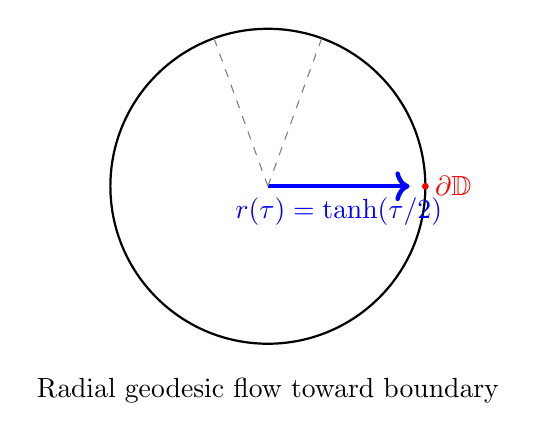
\begin{tikzpicture}[scale=2]
    \draw[thick] (0,0) circle (1);
    \draw[->, blue, ultra thick] (0,0) -- (0.9,0) node[midway, below] {$r(\tau) = \tanh(\tau/2)$};
    \filldraw[red] (1,0) circle (0.5pt) node[right] {$\partial\mathbb{D}$};
    \draw[gray, dashed] (0,0) -- (70:1);
    \draw[gray, dashed] (0,0) -- (110:1);
    \node at (0,-1.3) {Radial geodesic flow toward boundary};
\end{tikzpicture}
\caption{Proper time $\tau$ drives $r \to 1$. Dynamics freeze due to relativistic projection, not failure.}
\label{fig:radial_flow}
\end{figure}
\noindent\rule{16.5cm}{0.4pt}
\section{The Hidden Stage: Minkowski Space}

The hyperboloid model $X^2 + Y^2 - T^2 = -1$ ($T > 0$) in $(2+1)$-dimensional Minkowski space $ds^2 = dX^2 + dY^2 - dT^2$ is foundational. A radial geodesic:
\begin{equation*}
\Gamma(\tau) = (\sinh\tau, 0, \cosh\tau)
\end{equation*}
has proper time $\tau$. As $\tau \to \infty$, it approaches the null ray $(s, 0, s)$ without intersecting it.

Projecting to the Poincaré disk via $z = \frac{X + iY}{T + 1}$ gives:
\begin{equation*}
z(\tau) = i \tanh(\tau/2) \implies |z| \to 1 \text{ as } \tau \to \infty.
\end{equation*}
The Poincaré metric $ds_P = \frac{2|dz|}{1 - |z|^2}$ blows up near $|z|=1$ due to stretching of null asymptotics.

\begin{figure}[H]
\centering
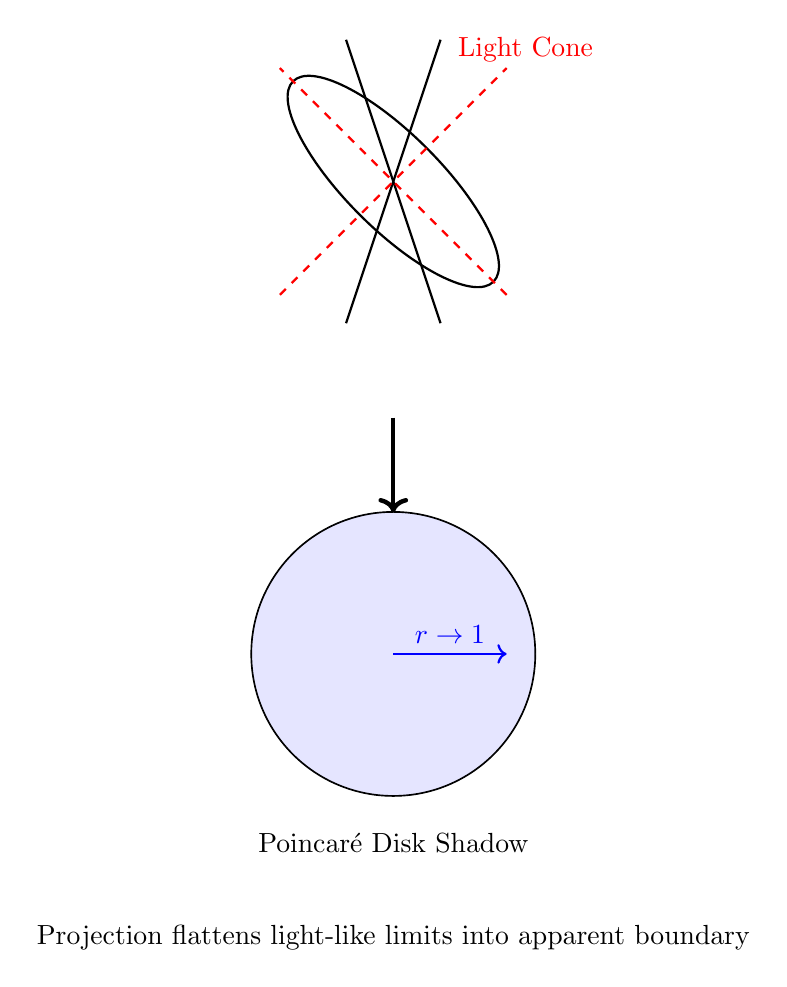
\begin{tikzpicture}[scale=1.2]
    % Hyperboloid
    \draw[thick, rotate around={45:(0,0)}] (0,0) ellipse (0.5 and 1.5);
    \draw[thick] (-0.5,-1.5) -- (0.5,1.5);
    \draw[thick] (0.5,-1.5) -- (-0.5,1.5);
    
    % Light cone
    \draw[dashed, red, thick] (-1.2,-1.2) -- (1.2,1.2);
    \draw[dashed, red, thick] (1.2,-1.2) -- (-1.2,1.2);
    \node[red] at (1.4,1.4) {Light Cone};
    
    % Projection arrow
    \draw[->, ultra thick] (0,-2.5) -- (0,-3.5);
    
% Poincare Disk below
\draw[thick] (0,-5) circle (1.5);
\draw[fill=blue!10] (0,-5) circle (1.5);
\draw[->, blue, thick] (0,-5) -- (1.2,-5) node[midway, above] {$r \to 1$};
\node at (0,-7) {Poincar\'e Disk Shadow};

% Annotation
    \node[align=center] at (0,-8) {Projection flattens light-like limits into apparent boundary};
\end{tikzpicture}
\caption{Hyperboloid (top) projects to Poincaré disk (bottom). Light cone (red) maps to $|z|=1$.}
\label{fig:projection}
\end{figure}

\section{Relativity in the Geometry Classroom}

As geodesics approach light-like behavior:
\begin{itemize}
    \item \textbf{Time dilation}: Proper time slows relative to lab frame.
    \item \textbf{Length contraction}: Objects contract along motion direction.
\end{itemize}
These effects manifest in projections as frozen clocks and flattened shapes.

\section{Boundary Point multiplicity}

Each boundary point corresponds to a null ray equivalence class. Geodesics $\Gamma_1$ and $\Gamma_2$:
\begin{equation*}
\Gamma_1(\tau) = (\sinh\tau, 0, \cosh\tau), \quad \Gamma_2(\tau) = (0, \sinh\tau, \cosh\tau)
\end{equation*}
project to $z=1$ and $z=i$, but perturbations show smooth endpoint transitions. The boundary catalogs light-like futures.

\section{Why This Isn't Taught}

Possible reasons:
\begin{itemize}
    \item Geometers avoid physics metaphors.
    \item Physicists rarely teach pure hyperbolic geometry.
    \item Textbooks prioritize formalism over intuition.
\end{itemize}

\section{Conclusion: A Bridge Between Worlds}

This framework uses existing math but shifts perspective. The boundary is a relativistic shadow, not infinity. Teaching this turns confusion into clarity.

\section*{Acknowledgments}
Thanks to coffee, curiosity, and students wondering why time stops.

\section*{Conflict of Interest}
The author declares none.

\section*{Funding}
No external funding.

\appendix

\section{Metric Degeneracy at the Light Cone}
On the light cone $X^2 + Y^2 = T^2$:
\begin{equation*}
ds_{\text{induced}}^2 = dX^2 + dY^2 - dT^2 = 0 \quad \text{(along generators)}.
\end{equation*}

\section*{Further Reading}
\begin{itemize}
    \item J. Ratcliffe, \emph{Foundations of Hyperbolic Manifolds}, Springer.
    \item R. Penrose, \emph{The Road to Reality}, Ch. 2, 16.
    \item W. Thurston, \emph{Three-Dimensional Geometry and Topology}, Vol. 1.
\end{itemize}

\end{document}
